\documentclass[12pt, a4paper]{article}

\usepackage[polish]{babel}
\usepackage[utf8]{inputenc}
\usepackage{polski}	
\frenchspacing	
\usepackage{graphics}
\usepackage{graphicx}

\title{\textbf{Obliczenia naukowe\\Lista 3}}
\author{Mateusz Kościelniak 244951\\}
\date{Listopad 2019}

\begin{document}

\maketitle

\newpage

\section{Zadanie 1, 2 i 3}
		
\subsection{Opis problemu}
Pierwsze trzy zadania polegały na zaimplementowaniu trzech metod,  takich jak:
\begin{itemize}  
\item metoda bisekcji 
\item metoda stycznych
\item metoda siecznych 
\end{itemize}
Zadaniem tych algorytmów jest znajdowanie miejsc zerowych funkcji z pewnym przybliżeniem.

\subsection{Rozwiązanie}
Moduł ze zródłami funkcji znajdują się w katalogu $.../FindRoots/src$ implementując metody  wzorowałem się na pseudokodzie znajdującym się na prezentacji z wykładu. Do modułu zostały dodane również testy jednostkowe, znajdują się one w katalogu $.../FindRoots/test$. Każda z funkcji została przetestowana pod kątem poprawności zwracanych wyników oraz błędów. 

\subsection{Wyniki}
Funkcje zostały zaimplementowane z powodzeniem, zostało to potwierdzone pozytywnym rezutatem testów jednostkowych.

\subsection{Wnioski}
Warto zwrócić uwagę  na pewne triki związane z implementacją algorytmów. Po pierwsze, punkt środkowy $c$ obliczany jest za pomocą instrukcji $c \leftarrow a + (b - a)/2$, co jest lepsze z numerycznego punktu widzenia (dodanie do poprzedniej wartości drobnej poprawki), wykonanie instrukcji $c \leftarrow (a + b)/2$ mogłoby spowodować, że w ekstremalnych przypadkach punkt $c$ znalazłby się poza przedziałem $[a, b]$. Po drugie, aby pozbyć się zbędnego mnożenia przy sprawdzeniu $f(a)f(c) < 0$, które mogłoby spowodować nadmiar lub niedomiar, zmianę znaku funkcji zbadano za pomocą nierówności $sign(w) \neq sign(u)$.


\newpage

\section{Zadanie 4}
		
\subsection{Opis problemu}
Zadanie polega na znalezieniu pierwiastka  równania $sin(x) - (\frac{x}{2})^{2} = 0$. Przy użyciu metod:
\begin{itemize}  
\item bisekcji (przedział początkowy $[1.5, 2.0]$)
\item stycznych (przybliżenie początkowe $x_{0} = 1.5$)
\item siecznych (przybliżenia początkowe $x_{0} = 1.0, x_{1} = 2.0$)
\end{itemize}
dla wszystkich metod:
$delta = 10^{-4}$, $epsilon = 10^{-4}$

\subsection{Rozwiązanie}
Do rozwiązania zadania użyłem wcześniej zaimplementowanych funkcji z modułu FindRoots, z zadanymi w treści zadania parametrami wejściowymi. Musiałem również obliczyć pochodną funkcji $f$ która wyniosła $f'(x) = cos(x)-\frac{x}{2}$

\subsection{Wyniki}
\begin{table}[h]
        \centering
        \footnotesize
        \renewcommand{\arraystretch}{1.5}
\begin{tabular}{c|c|c|c|c} 
Metoda & $x_{0}$ & $f(x_{0})$ & Liczba iteracji & Flaga błędu\\
\hline
Bisekcji &1.9337539672851562&-2.7027680138402843e-7& 16 & 0 \\
Stycznych &1.933753779789742&-2.2423316314856834e-8& 4 & 0 \\
Siecznych &1.933753644474301&1.564525129449379e-7& 4 & 0 \\
\end{tabular}
\caption{Szukanie rozwiązań równania $cos(x)-\frac{x}{2} = 0$, trzema metodami.}
\end{table}

\subsection{Wnioski}
Wszystkie wyniki są poprawne z dokładnością co do epsilona. Widzimy jednak 
dużą różnicę w liczbie wykonanych iteracji pomiędzy metodą bisekcji a metodami stycznych i siecznych, takie  wyniki odzwierciedlają teoretyczną zbieżność tych metod, bisekcja posiada liniowy współczynnik zbieżności, natomiast metoda stycznych kwadratowy a metoda siecznych jest tak tzw. metodą superliniową z współczynnikiem zbieżności wynoszącym $\approx1.618$

\newpage

\section{Zadanie 5}

\subsection{Opis problemu}
Znalezienie wartości zmiennej $x$, dla której przecinają sie wykresy funkcji $y = 3x$ i $y = e^{x}$, przy użyciu metody  bisekcji.

\subsection{Rozwiązanie}
Problem sprowadza się do zalezienia wszystkich rozwiązań równania $e^x - 3x = 0$, W tym celu zaimplementowana została funkcja $f(x) = e^x - 3x$. Przedziały początkowe wyznaczyłem na podstawie wykresu.

\begin{figure}[h]
\centering
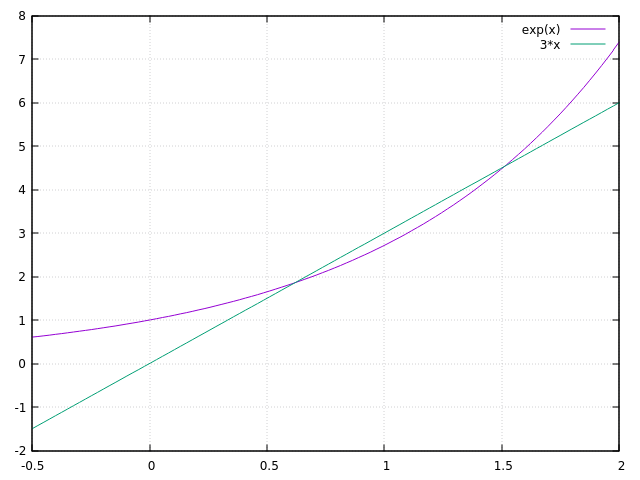
\includegraphics[width=0.9\textwidth]{zad5.png}\hfill
\end{figure} 

Wyniosły one kolejno $[0.0,1.1]$ oraz $[1.0, 2.0]$. Za dokładność obliczeń przyjąłem $\delta=10^{-4}$ oraz $\epsilon=10^{-4}$.

\newpage

\subsection{Wyniki}
\begin{table}[h]
        \centering
        \footnotesize
        \renewcommand{\arraystretch}{1.5}
\begin{tabular}{c|c|c|c} 
Przedział & $x_{0}$ & $f(x_{0})$ & Liczba iteracji \\
\hline
$[0.0, 1.0]$ & 0.619140625 & -9.066320343276146e-5 & 9 \\
$[1.0, 2.0]$ & 1.5120849609375 & -7.618578602741621e-5 & 13 \\
\end{tabular}
\caption{Szukanie miejsca przecięcia funkcji $y = e^{x}$, $y = 3x$ metodą bisekcji.}
\end{table}

\subsection{Wnioski}
Największym problemem w tym zadaniu był dobór rzedziałów początkowych, lecz znając przebieg funkcji $y = 3x$ i $y = e^{x}$ ($e^{x}$ rośnie bardzo szybko względem $3x$), po kilku próbach udało mi się narysować wykres z odpowiednią dokładnością aby wybrać przedziały.  Wybranie przedziałów jest kluczowym etapem w rozwiązaniu tego typu zadania, aby otrzymać poprawny wynik musimy mieć pewność, że funkcja ma tylko jedno miejsce zerowe w przedziale, do tego potrzebna jest analiza funkcji.

\newpage

\section{Zadanie 6}

\subsection{Opis problemu}
Znalezienie miejsc zerowych funkcji $f_{1}(x) = e^{1-x}-1$  oraz $f_{2}(x) = e^{1-x}-1$ za pomocą wszystkich trzech metod zaimplementowanych z zadaniach 1-3. Dokładność obliczeń to $\delta=10^{-5}$ oraz $\epsilon=10^{-5}$.
Należało również sprawdzić zachowanie metody newtona dla funkcji $f_{1}$ i $f_{2}$ z przybliżeniem początkowym $x_{0} \in{(1, \infty]}$ oraz odpowiedzieć na pytanie czy można wybrać przybliżenie początkowe $x_{0}=1$ dla $f_{2}$.

\subsection{Rozwiązanie}
Wybierając punkty początkowe znów posłużyłem sie wykresem tak jak w zadaniu poprzednim.

\begin{figure}[h]
\centering
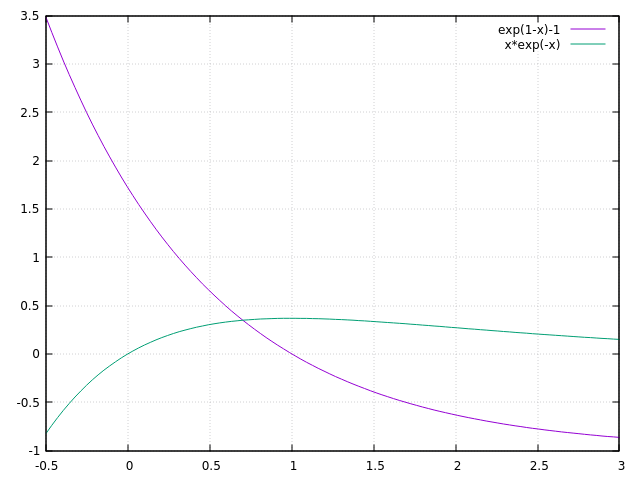
\includegraphics[width=0.9\textwidth]{zad6.png}\hfill
\end{figure} 

Patrząc na wykres możemu oszacować miejsce zerowe $f_{1}$ na 1.0 a $f_{2}$ na 0.0
Na tej podstawie dobrałem parametry do funkcji, możemy je zobaczyć poniżej, w tabeli w sekcji z wynikami. Musiałem również obliczyć pochodne obydwóch funkcji, a do rozwiązania zadania użyłem wcześniej zaimplementowane algorytmy.

\newpage

\subsection{Wyniki}

\begin{table}[h]
        \centering
        \footnotesize
        \renewcommand{\arraystretch}{1.5}
\begin{tabular}{c|c|c|c|c} 
Funkcja & Przedział & $x_{0}$ & $f(x_{0})$ & Iteracje \\
\hline
$f_{1}$ & $[0.0, 1.5]$ & 1.0000076293945312 & -7.6293654275305656e-6 & 16 \\
$f_{2}$ & $[-0.5, 1.0]$ & -7.62939453125e-6 & -7.629452739132958e-6 & 16 \\
$f_{2}$ & $[-0.5, 1000.0]$ & 499.75 & 4.571781560397468e-215 & 1 \\
\end{tabular}
\caption{Pierwiastki funkcji metodą bisekcji.}
\end{table}

\begin{table}[h]
        \centering
        \footnotesize
        \renewcommand{\arraystretch}{1.5}
\begin{tabular}{c|c|c|c|c|c} 
Funkcja & Przybliżenie & $x_{0}$ & $f(x_{0})$ & Iteracje\\
\hline
$f_{1}$ & $0.5$ & 0.9999999998878352 & 1.1216494399945987e-10 & 4 \\
$f_{2}$ & $-0.5$ & -3.0642493416461764e-7 & -3.0642502806087233e-7 & 4 \\
\end{tabular}
\caption{Pierwiastki funkcji metodą stycznych.}
\end{table}

\begin{table}[h]
        \centering
        \footnotesize
        \renewcommand{\arraystretch}{1.5}
\begin{tabular}{c|c|c|c|c} 
Funkcja & Przybliżenia & $x_{0}$ & $f(x_{0})$ & Iteracje \\
\hline
$f_{1}$ & $[-1.0, 1.5]$ & 0.9999908642801245 & 9.135761606327009e-6 & 5 \\
$f_{2}$ & $[-1.0, 0.5]$ & -1.1737426154042664e-6 & -1.1737439930768023e-6 & 7 \\
\end{tabular}
\caption{Pierwiastki funkcji metodą siecznych.}
\end{table}

\begin{table}[h]
        \centering
        \footnotesize
        \renewcommand{\arraystretch}{1.5}
\begin{tabular}{c|c|c|c|c|c} 
Funkcja & Przybliżenia & $x_{0}$ & $f(x_{0})$ & Iteracje & Błąd \\
\hline
$f_{1}$ & $2.0$ & 0.9999999810061002 & 1.8993900008368314e-8 & 5 & 0 \\
 & $5.0$ & 0.9999996427095682 & 3.572904956339329e-7 & 54 & 0\\
 & $6.0$ & 0.9999999573590406 & 4.264096031825204e-8 & 147  & 0 \\
 & $8.0$ & - & - & - & 1 \\
\hline
$f_{2}$ & $1.0$ & - & - & - & 2 \\
 & $2.0$ & 14.398662765680003 & 8.036415344217211e-6 & 10 & 0 \\
 & $5.0$ & - & - & - & 2 \\
 & $6.0$ & 14.398662765680003 & 4.699833827208111e-6 & 8 & 0 \\
\end{tabular}
\caption{Pierwiastki funkcji metodą stycznych - 2 część zadania.}
\end{table}


\newpage

\subsection{Wnioski}
Metody bisekcji, stycznych oraz siecznych dla funkcji $f_{2}$ przy nieostrożnie dobranym przybliżeniu początkowym, mogą zwrócić pierwiastki już w pierwszejiteracji, które nie są miejscai zerowymi, dzieje się tak ponieważ funkcja zbiega do zera dla coraz większych argumentów co powoduje, że funkcja przyjmuje wartości poniżej zakładanej dokładności w miejscach które niekoniecznie są jej pierwiastkami. W metodzie stycznych jeśli przybliżenie początkowe będzie bardzo bliskie zeru to obliczenia nie będą kontynuowane. W algorytmie stycznych dodatkowo występuje taka sytuacja, że jeśli szybkośc zmiany funkcji jest bardzo mała to obliczenia nie będą kontynuowane,możemy to zobaczyć w Tabeli 5.\\

Dla metody stycznych wybranie wartości $x_{0} = 1$ dla funckji $f_{2}$ spowoduje wyzerowanie się pochodnej oraz wyrzucenie błędu o treści pochodna bliska zeru, natomiast dla wartości $x_{0} > 1$, funkcja metoda nie zbiega do faktycznego zera funkcji tylko znajduje wartość bliską zeru odległą od rzeczywistego zera funkcji z tego powodu, że $\lim\limits_{x \to \infty} f_{2}(x) = 0$. Dla funkcji $f_1$ i $x_0 \in [1,\infty]$ mamy analogiczną sytuacje, funkcja ta bardzo wolno maleje , co za tym idzie pochodna staje się bardzo bliska zeru, drugim niebezpieczeństwem jest to, że liczba iteracji znacznie rośnie ($x_0 = 8$ i 10 mln iteracji nie dostajemy wyniku) aż w końcu metoda staje się rozbieżna.\\

Wnioskiem płynącym z tego zadania jest to, że przy obliczaniu pierwiastków 
równania istotny jest nie tylko wybór najlepszego algortmu, ale również analiza funkcji i dopasowanie algorytmu pod kątem tejże funkcji oraz wybór odpowiednich przybliżeń początkowych.
\end{document}
